\subsection{LoginScreen}

Der \lstinline{Login-Screen} dient als - wie der Name schon verrät - Anmelde-Maske der App, über 
welche sich bereits bestehende Nutzer anmelden können, um auf die Dienste von Sokka zugreifen und
Bestellungen aufgeben können.

Wie jedes Widget, mit dem der Nutzer interagieren soll, ist auch der Login-Screen ein Stateful 
Widget, schließlich sollen hier die benötigten Anmeldedaten eingegeben und per Druck eines Buttons
zur Verifizierung an den Server gesendet werden.

Für die Eingabe eines vom Nutzer abhängigen Textes werden ein \lstinline{TextFormField}-Widget
und ein sogenannter \lstinline{TextEditingController}, der die Eingabe des Feldes überwacht,
benötigt.

Damit der Text innerhalb des Screens als Wert verfügbar und verwendbar ist, wird dieser vom entsprechenden
Controller in die passende Klassenvariable geschrieben.\\
So können die eingegebenen Daten in weiterer Folge per Request an den Server gesendet und überprüft werden.

Bei erfolgreicher Anmeldung werden sowohl der Cookie-Storage als auch der Menu- und
Product-Controller per Funktion initialisiert.

\begin{code}[h]
    \centering
    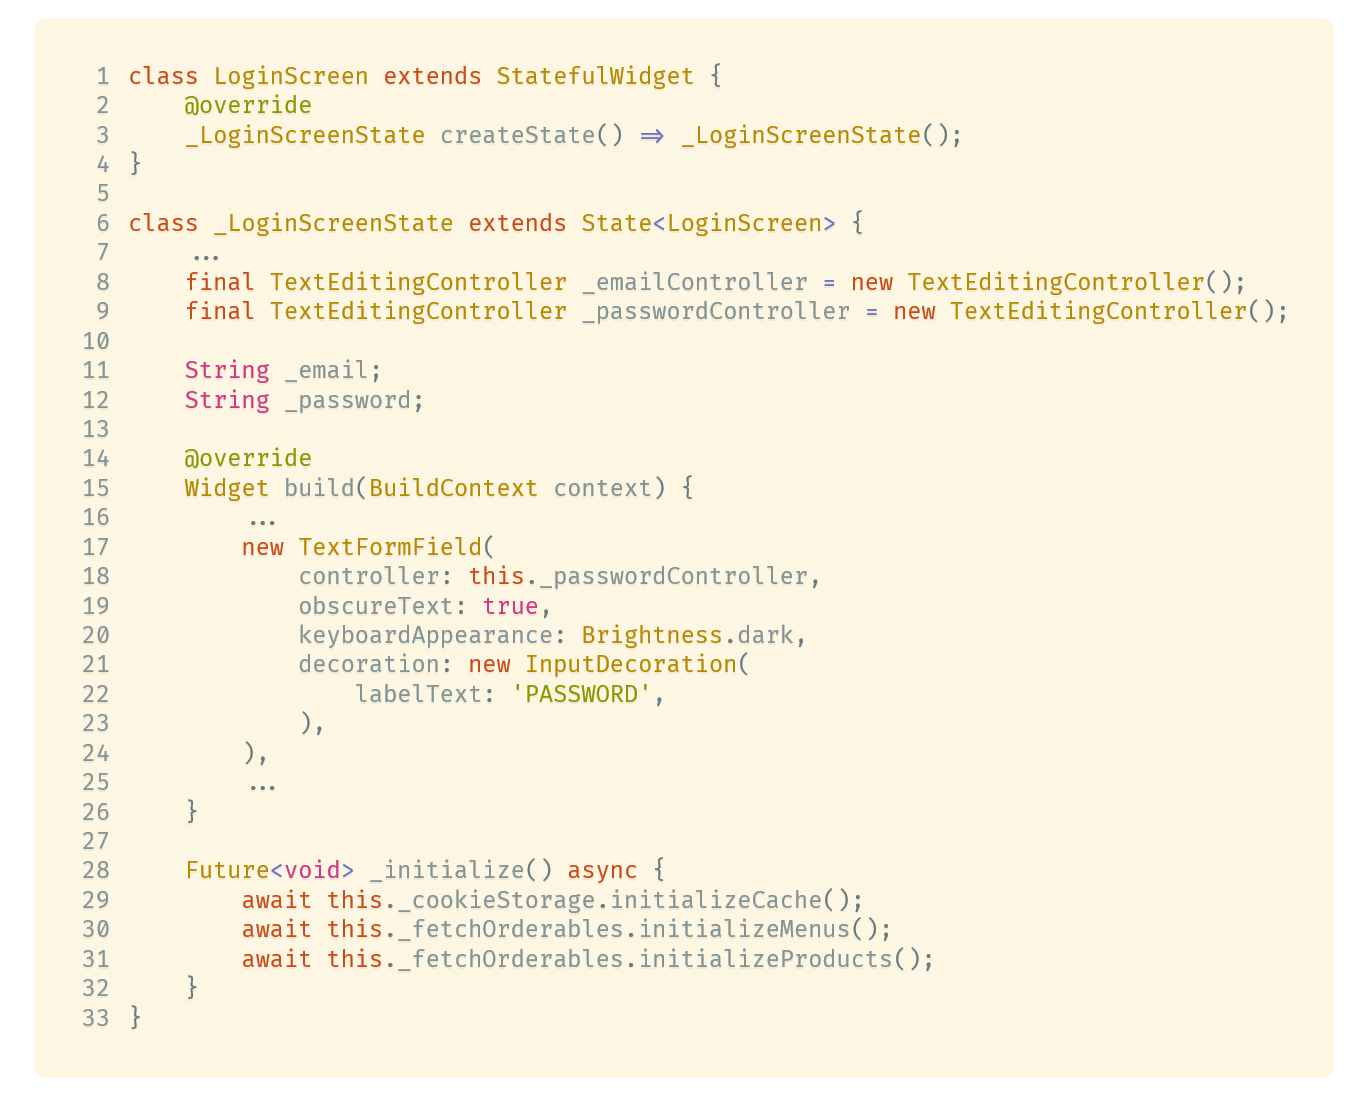
\includegraphics[width=1\textwidth]{images/Client/screens/login/loginScreen.png}
    \caption{Login-Screen als Stateful Widget mit \lstinline{TextFormFields} und \lstinline{TextEditingControllers} für E-Mail und Passwort}
\end{code}

\newpage